\documentclass[10pt]{article}
\usepackage[dvips]{graphicx}
\usepackage[small,bf]{caption}
\usepackage[american]{varioref}
\usepackage{wrapfig}
\usepackage{html}

% Margin adjustments.  vmargin.sty interacts badly with page numbers at
% the bottom of the page, so we just code the number manually here.

\oddsidemargin  0pt
\evensidemargin 0pt
\topmargin      0.5ex
\hoffset        0 in
\textwidth      6.5 in
\textheight     9 in

% Style adjustments.

% Fix placement of figures & tables.  This keeps latex from shoving big
% floats to the end of a document when they are somewhat big, which it will
% do even if you put [htb] as the argument.

\setcounter{topnumber}{1}
\setcounter{bottomnumber}{1}
\def\topfraction{1.0}
\def\bottomfraction{1.0}
\def\textfraction{0.0}
\def\floatpagefraction{0.9}

%begin{latexonly}

\raggedbottom

\def\captionfont{\itshape}              % Use italic font for captions.

\makeatletter

\setlength{\parindent}{0 pt}            % Unindented paragraphs, separated ...
\setlength{\parskip}{1.3 ex}            % ... by roughly one blank line.
\setlength{\partopsep}{-0.5 ex}

\renewcommand{\section}{\@startsection%
  {section}{1}{0pt}{-1.8ex \@plus -1ex \@minus -.2ex}%
  {0.8ex}{\normalfont\Large\bfseries}}

\renewcommand{\subsection}{\@startsection%
  {subsection}{2}{0pt}{-2ex \@plus 1ex \@minus -.2ex}%
  {0.8ex}{\slshape\large\bfseries}}

\renewcommand{\subsubsection}{\@startsection%
  {subsubsection}{3}{0pt}{-1.5ex \@plus 1ex \@minus -.2ex}%
  {0.5ex}{\slshape\normalsize\bfseries}}

\newcommand{\tightspacing}{\renewcommand{\baselinestretch}{0.85}}
\newcommand{\regularspacing}{\renewcommand{\baselinestretch}{1.0}}

\makeatother

%end{latexonly}

% Miscellaneous macros.

\newcommand{\fig}[2][]{\def\fboxsep{0pt}\fbox{\includegraphics[#1]{#2}}}
\newcommand{\figNB}[2][]{\includegraphics[#1]{#2}}
\newcommand{\url}[1]{\texttt{#1}}
\newcommand{\menu}[1]{\textsf{\textbf{#1}}}
\newcommand{\class}[1]{\textsf{#1}}
\newcommand{\attrib}[1]{\textsf{#1}}
\newcommand{\attribtype}[1]{\textsf{#1}}

\begin{document}

%=============================================================================
% Title page
%=============================================================================

\title{\textbf{A Notation for Describing Model Representations\\
Intended for XML Encoding}}

\author{Michael Hucka\\[2pt]
\normalsize\texttt{mhucka@bbb.caltech.edu}\\[-2pt]
\normalsize ERATO Kitano Systems Biology Project\\[-2pt]
\normalsize Control and Dynamical Systems 107-81\\[-2pt]
\normalsize California Institute of Technology, Pasadena, CA 91125}

\date{Version of \today{}}

\maketitle

%=============================================================================
\section{Introduction} 
\label{sec:introduction}
%=============================================================================

% Need to mention that explaining xml is beyond scope

One component of the ERATO Kitano Systems Biology Project is the creation
of a workbench that provides interoperability between a number of
simulation packages.  Developing a framework for simulator interoperability
requires defining a language for communicating data between software
packages.  Defining this language requires first establishing a notation
that humans can use to describe the data structures involved.

I propose a simple notation to be used for describing data structures that
are intended to be encoded using XML, the Extensible Markup Language~(Bosak
and Bray, 1999; Bray, Paoli and Sperberg-McQueen, 1998; Fallside, 2000).
The notation is based partly on a small subset of UML, the Unified Modeling
Language~(Eriksson, 1998; Oestereich, 1999), a visual language for
specifying software systems.  There are two main advantages to using UML
for defining data structures.  First, the visual representations are
generally easier to read and understand by readers who are not computer
scientists.  Second, the visual notation is implementation-neutral---the
defined structures can be encoded in any concrete implementation language,
not just XML but other formats as well, making the UML-based definitions
more useful and flexible.

Readers do not need to know UML in advance; this document provides
descriptions of all the constructs needed.  The notation presented here can
be expressed not only in graphical diagram form (which is what UML is all
about) but also in textual form, allowing descriptions to be easily written
in a text editor and sent as plain-text email.  I provide a systematic
method for translating the visual diagrams into XML Schemas.

It is important to note that the vocabulary of the notation is purposefully
limited to only a handful of constructs.  It is explicitly not intended to
cover the full power of UML or XML.  This limited vocabulary is
nevertheless sufficient for the applications to which it has been applied
so far in the Systems Biology Project.


%=============================================================================
\section{Representing Object Structures in XML}
\label{sec:representing}
%=============================================================================

An XML data stream consists of two basic parts: (1) an optional vocabulary
and structure definition (either in the form of a \emph{Document Type
  Definition} or an \emph{XML Schema}), and (2) the body of the stream,
containing data objects organized using this definition.  XML provides the
ability to define hierarchically nested data structures; this works well
for representing object-oriented data because objects are basically nested
field-value structures.  Non-tree graph structures can also be encoded in XML.

An \emph{XML Schema} (Biron and Malhotra, 2000; Fallside, 2000; Thompson et
al., 2000) specifies the types of objects allowed in an XML data stream, as
well as how the objects and their fields can be organized and the types of
the values that can be assigned to the object fields.  It provides more
expressive power than the alternative mechanism for defining the structures
of XML streams, the document type definition (DTD).

While it is extremely powerful, the XML Schema language (and for that
matter, the DTD language) is complicated enough that it is not suitable as
a descriptive specification language for humans communicating about data
structures used in a software project.  A more suitable language is UML, an
industry-standard visual language, but there currently does not exist an
agreed-upon approach for translating UML representations into XML Schemas.
One of the goals of this document is to present one such approach for a
small set of common cases.


%-----------------------------------------------------------------------------
\subsection{Basis of the Approach}
\label{sec:xml}
%-----------------------------------------------------------------------------

\begin{wrapfigure}[6]{r}{1.75 in}
  \begin{center}
    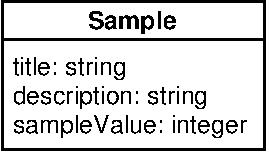
\includegraphics[scale = 0.7]{sampleschema.eps}
  \end{center}
\end{wrapfigure}
An instance of a data object is always constructed according to a blueprint
or \emph{class} definition that defines the internal structure of the
object.  The ``structure'' is its attributes and the types of data values
that are permitted to be stored in the attributes.  In UML notation, a
class is represented as a box with a title and a list of attributes below
it, as in the example shown at right.  The example shows an object class
named \class{Sample} having three attributes: \attrib{title},
\attrib{description}, and \attrib{sampleValue}.

In XML terminology, objects in an XML document or data stream are referred
to as \emph{elements}.  Elements can contain values that may themselves be
other elements, and elements can have annotations in the form of
attributes.  The following piece of XML illustrates the different parts of
an XML representation:

\begin{quote}
  \begin{small}
    \tightspacing
\begin{verbatim}
<element1 attributeA="attributeA-value">element1-value</element1>
<element2 attributeB="attributeB-value" attributeC="attributeC-value">
  <element3>element3-value</element3>
  <element4 attributeD="attributeD-value">element4-value</element4>
</element2>
\end{verbatim}
    \regularspacing
  \end{small}
\end{quote}

The example above shows four separate elements.  Some of the elements have
attributes (\texttt{element1}, \texttt{element2}, \texttt{element4}), while
some do not (\texttt{element3}).  Some of the elements have simple values
(\texttt{element1}, \texttt{element3}, \texttt{element4}), while the other
one (\texttt{element2}) contains two other elements (\texttt{element3},
\texttt{element4}) as its value.

XML element attributes are name-value pairs that can only be used to hold
simple (scalar) values.  Storing a value that is more structured than a
simple value (e.g., another object) requires the use of a subelement.  When
encoding a UML data structure in XML, an attribute in the UML structure may
or may not be made into an XML element attribute.  Indeed, one of the first
questions that needs to be answered when developing an XML format is: what
should be stored as element attributes, and what should be stored as
element values?

Unfortunately, there appears to be no agreed-upon rule to answer this
question.  Some authors lean towards using elements to store ``real''
content and attributes to put ``invisible annotations'' on the elements
(St.~Laurent, 2000).  But this is by no means universally accepted, as is
clear from the different views summarized by Cover~(2000), and one of the
original architects of XML has stated that ``I've never heard a convincing
universal decision procedure for what should be an element and what an
attribute''~(Bray, 1998).  Instead of treating element attributes as
invisible annotations, it is also valid to treat XML elements as data
objects and element attributes as field values of those data objects.  To
put these differences into concrete terms, here are two samples of XML that
can both be taken to express the same data:
\begin{center}
  \setlength{\tabcolsep}{20 pt}
  \tightspacing
  \small
  \begin{tabular}{@{}ll@{}}
    \begin{minipage}[t]{1.5 in}
      \begin{tabbing}
        xx\=\kill
        \verb|<Sample>|\\
        \>\verb|<title>My title</title>|\\
        \>\verb|<description>My description</description>|\\
        \>\verb|<sampleValue>42</sampleValue>|\\
        \verb|</Sample>|
      \end{tabbing}
    \end{minipage}
    &
    \begin{minipage}[t]{1.5 in}
      \begin{tabbing}
        xSample \=\kill
        \verb|<Sample title="My title"|\\
                \>\verb|description="My description"|\\
                \>\verb|sampleValue="42"/>|
      \end{tabbing}
    \end{minipage} \\ \\
    \emph{Approach 1} & \emph{Approach 2}
  \end{tabular}
\end{center}
The second approach has the advantage of being a more compact encoding.
The approach also leads to a direct correspondence between object
attributes and XML element attributes: when we speak about an ``attribute''
of an object, the corresponding XML construct is an attribute on an
element, as in the example on the right above.

For these reasons, the notation presented here is based on the second
approach.


%=============================================================================
\section{The UML-Based Notation and Its Textual and XML Forms}
\label{sec:schemas}
%=============================================================================

The following example presents an example object class definition in the
UML-style notation adopted here, along with its representation in a textual
form and in XML Schema syntax:

\begin{center}
  \tightspacing
  \small
  \setlength{\tabcolsep}{10 pt}
  \begin{tabular}{@{}lll@{}}
    \begin{minipage}[b]{1.3 in}
      \raisebox{-2ex}{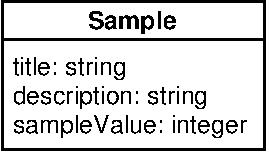
\includegraphics[scale = 0.7]{sampleschema.eps}}
    \end{minipage}
  &
    \begin{minipage}[b]{1.5 in}
      \begin{tabbing}
	sampleValuexx\=\kill
        \class{Sample}\\
	\rule[0.5 ex]{1.3 in}{0.005in}\\
        \attrib{title}:\>\attribtype{String}\\
        \attrib{description}:\>\attribtype{XHTML}\\
        \attrib{sampleValue}:\>\attribtype{Integer}
      \end{tabbing}
    \end{minipage}
  &
    \begin{minipage}[b]{3 in}
      \begin{tabbing}
        xx\=\kill
        \verb|<complexType name="Sample">|\\
        \>\verb|<attribute name="title" type="string"/>|\\
        \>\verb|<attribute name="description" type="string"/>|\\
        \>\verb|<attribute name="sampleValue" type="integer"/>|\\
        \verb|</complexType>|
      \end{tabbing}
    \end{minipage}
    \\
    \\
    \emph{UML Form} & \emph{Textual Form} & \emph{XML Schema}
  \end{tabular}
  \regularspacing
\end{center}

All three forms define the same data structure: a class \class{Sample} of
of objects having three attributes.  The components are named according to
a particular naming convention:
\begin{itemize}
  
\item The name of the class must begin with an uppercase letter, can
  contain letters, numerals and underscore characters, and (due to
  limitations in the software tools we are using) cannot have space
  characters in them.  Words within the names should each be capitalized.
  
\item Attribute names generally begin with a lowercase letter but otherwise
  follow the convention for object class names; for example, an attribute
  might be named \attrib{sampleValue}.  An exception to this rule can be
  made when the attribute name begins with a word that is normally
  capitalized, such as an acronym (e.g., ``\attrib{IDReference}'').

\end{itemize}

Attributes are typed.  There are a number of categories of possible
datatypes, as explained in
Sections~\ref{sub:simple-attributes}--\ref{sub:list-attributes}.  In the
notation used here, the type specifier is written after the name of the
attribute, as in, for example, \attrib{title: String}.  This convention is
commonly used in UML textbooks (e.g., Eriksson and Penker, 1998).  An
alternative UML style puts the type specifier before the attribute name, as
in, for example, \attrib{String title}.


%-----------------------------------------------------------------------------
\subsection{Simple Attribute}
\label{sub:simple-attributes}
%-----------------------------------------------------------------------------

A simple attribute is one having a simple data value, for example a number
or a string.  All three of the attributes shown in the \class{Sample}
example above are simple attributes.  The set of simple types that are
permitted is the set defined by the XML Schema standard, plus simple types
derived from the built-in ones.  Figure~\ref{fig:simple-types} lists the
simple types built into XML Schema.

\begin{figure}
  \centering
  \small
  \begin{tabular}{@{}ll@{}}
    \textbf{Type} & \textbf{Example(s)} \\
         string		& \texttt{Confirm this is electric} \\
         boolean 	& \texttt{true, false, 1, 0} \\
         float		& \texttt{-INF, -0, 0, 1.7E-2, 3, INF, NaN} \\
         double		& \texttt{-INF, -0, 0, 1.7E-2, 3, INF, NaN} \\
         decimal	& \texttt{-1.23, 0, 123.4, 1000.00} \\
         timeInstant	& \texttt{1999-05-31T13:20:0.0-05:00} \\
         timePeriod	& \texttt{1999-05-31T13:20} \\
         month		& \texttt{1999-05} \\
         year		& \texttt{1999} \\
         century	& \texttt{19} \\
         recurringDate	& \texttt{--05-31} \\
         recurringDay	& \texttt{----31} \\
         timeDuration	& \texttt{P1Y2M3DT10H30M12.3S} \\
         recurringDuration	& \texttt{--05-31T13:20:00} \\
         binary		& \texttt{100010} \\
         uriReference	& \texttt{http://www.me.com/x.html\#id5} \\
         ID             & \texttt{m32} \\
         IDREF \\
         ENTITY \\
         NOTATION \\
         language \\
         IDREFS         & \texttt{m32 m33 m34 m35} \\
         ENTITIES \\
         NMTOKEN 	& \texttt{US} \\
         NMTOKENS		& \texttt{US UK} \\
         Name		& \texttt{shipTo} \\
         QName		& \texttt{po:Address} \\
         NCName		& \texttt{Address} \\
         integer		& \texttt{-126789, -1, 0, 1, 126789} \\
         nonPositiveInteger		& \texttt{-126789, -1, 0} \\
         negativeInteger		& \texttt{-126789, -1} \\
         long		& \texttt{-1, 12678967543233} \\
         int		& \texttt{-1, 126789675} \\
         short		& \texttt{-1, 12678} \\
         byte		& \texttt{-1, 126} \\
         nonNegativeInteger		& \texttt{0, 1, 126789} \\
         unsignedLong		& \texttt{0, 12678967543233} \\
         unsignedInt		& \texttt{0, 1267896754} \\
         unsignedShort		& \texttt{0, 12678} \\
         unsignedByte		& \texttt{0, 126} \\
         positiveInteger		& \texttt{1, 126789} \\
         date		& \texttt{1999-05-31, ---05} \\
         time		& \texttt{13:20:00.000-05}:00
  \end{tabular}
  \caption{Simple types built into XML Schema, according to the W3C Working
    Draft of 7 April 2000 (Biron and Malhotra, 2000).}
  \label{fig:simple-types}
\end{figure}


%-----------------------------------------------------------------------------
\subsection{Complex Attribute}
\label{sub:complex-attributes}
%-----------------------------------------------------------------------------

An attribute can be a container for a collection of attributes under a
common heading.  In that case, the attribute's value is not a simple
scalar; it is therefore called a complex attribute.  This is roughly
equivalent to a ``struct'' in the language C.

The following is an example involving a complex type, shown in the textual
notation form:

\begin{center}
  \setlength{\tabcolsep}{40 pt}
  \tightspacing
  \small
  \begin{tabular}{@{}cc@{}}
    \begin{minipage}{1.6in}
      \begin{tabbing}
        AttrCTypexx\=\kill
        \class{MyClass}\\
        \rule[0.5 ex]{1.4 in}{0.005in}\\
        \attrib{attributeA}:\>\attribtype{String}\\
        \attrib{attributeB}:\>\attribtype{String}\\
        \attrib{attributeC}:\>\attribtype{AttrCType}
      \end{tabbing}
    \end{minipage}
    & 
    \begin{minipage}{1.6in}
      \begin{tabbing}
        yetanotherattributexxx\=\kill
        \class{AttrCType}\\
        \rule[0.5 ex]{1.75 in}{0.005in}\\
        \attrib{anotherAttribute}:\>\attribtype{Integer}\\
        \attrib{yetAnotherAttribute}:\>\attribtype{Float}
      \end{tabbing}
    \end{minipage}
  \end{tabular}
  \regularspacing
\end{center}

The meaning of the above is: \class{MyClass} consists of three attributes
\attrib{attributeA}, \attrib{attributeB} and \attrib{attributeC}.  The last
attribute is actually a class containing two other attributes.  In a
programming language, given an object \texttt{obj} of class
\class{MyClass}, the attributes might be accessed as
\begin{small}
  \tightspacing
\begin{verbatim}
    obj.attributeA
    obj.attributeB
    obj.attributeC.J
    obj.attributeC.K
\end{verbatim}
  \regularspacing
\end{small}

In UML, a complex type must be defined as a separate class.  The following
is an example UML diagram representing the same data structures as above:

\begin{center}
  \figNB[scale = 0.7]{someschema-uml.eps}
\end{center}

The meaning of the above is: \class{MyClass} consists of all the attributes
within the box of the class definition, \emph{plus} the attribute
\attrib{attributeC}, which is of a complex type called \class{AttrCType}.
By UML convention, the attribute \attrib{attributeC} does not appear in the
\class{MyClass} box itself.  Therefore, in reading UML diagrams containing
associations between classes, it is important to count \emph{both} the
attributes within the class box as well as the attributes shown on the
association lines.

The only naming convention defined here for complex types is that the names
should begin with a capital letter.  However, it is a good idea to make the
name of a complex type reflect the attribute to which it is connected.
(E.g., for an attribute named \attrib{version}, the complex type might be
named \class{Version}.)

As explained in the previous section, simple attribute types translate into
element attributes in XML.  Complex types translate directly into the
\attrib{complexType} element in XML Schemas.  But there is some flexibility
in how to compose complex types within an object definition.  The approach
taken here is to use a nested XML element named after the name of the link
between the main class and the subsidiary class.  The following is an
example illustrates the idea for \class{MyClass}:
\begin{small}
  \tightspacing
\begin{verbatim}
    <MyClass attributeA="foo" attributeB="bar">
      <attributeC>
        <AttrCType anotherAttribute="2" yetAnotherAttribute="4.3"/>
      </attributeC>
    </MyClass>
\end{verbatim}
  \regularspacing
\end{small}
Note how the attribute \attrib{attributeC} is written out as a separate XML
element container, and the class name \class{AttrCType} is the name of the
subelement within \attrib{attributeC}.  Although it may seem unnecessary to
have a second level of nesting for a single subelement, this approach
extends nicely to situations where there may be lists of subelements, as
discussed in Section~\ref{sub:list-attributes}.  Using the same notation in
both cases is best for consistency.

Finally, here is the corresponding XML Schema definition:
\begin{small}
  \tightspacing
\begin{verbatim}
    <xsd:schema xmlns:xsd="http://www.w3.org/1999/XMLSchema">
    
    <xsd:complexType name="AttrCType">
      <xsd:attribute name="anotherAttribute" type="xsd:integer"/>
      <xsd:attribute name="yetAnotherAttribute" type="xsd:float"/>
    </xsd:complexType>
    
    <xsd:attribute name="attributeA" type="xsd:string"/>
    <xsd:attribute name="attributeB" type="xsd:string"/>
    <xsd:element   name="attributeC" minOccurs="1" maxOccurs="1">
      <xsd:complexType>
        <xsd:element name="AttrCType" type="AttrCType" minOccurs="0" maxOccurs="1"/>
      </xsd:complexType>
    </xsd:element>
    
    </xsd:schema>
\end{verbatim}
  \regularspacing
\end{small}
In this XML Schema, \attrib{attributeC} is defined as an element with
constraints (the \verb|minOccurs| and \verb|maxOccurs| terms in the schema
above) that say, in effect, ``there must be exactly one of these present''.
This produces the \verb|<attributeC>...</attributeC>| nested pair in the
\class{MyClass} example above.  The contents within this nested pair are
limited to at most one instance of an element of the form
\verb|<AttrCType anotherAttribute=... />|.


%=============================================================================
\subsection{Containers with Values}
%=============================================================================

In addition to the way that simple and complex types are used here, XML
also allows elements to have values aside from other elements and
attributes.  This was shown in the examples in Section~\ref{sec:xml}.  In
the translation approach adopted here, most objects are encoded as
attributes on an XML element.  However, it is useful to be able to denote a
type which is a container for a value, as in the following example:
\begin{small}
  \tightspacing
\begin{verbatim}
    <SomeClass title="This is a title">
      <bigValue>
               This is some long value, maybe something that has
               some <b>HTML</b> formatting tags embedded within it, 
               or maybe something that's just too awkward to put all
               inside an attribute value.
      </bigValue>
    </SomeClass>
\end{verbatim}
  \regularspacing
\end{small}
Expressing this in UML requires a special notation.  The following
illustrates the modified UML notation adopted here:
\begin{center}
  \tightspacing
  \small
  \setlength{\tabcolsep}{10 pt}
  \begin{tabular}{@{}ll@{}}
    \begin{minipage}[b]{3 in}
      \raisebox{2ex}{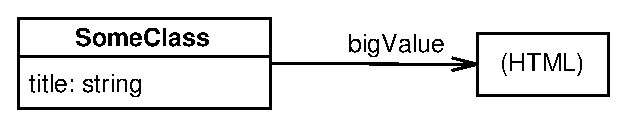
\includegraphics[scale = 0.7]{container.eps}}
    \end{minipage}
  &
    \begin{minipage}[b]{1.5 in}
      \begin{tabbing}
	sampleValuexx\=\kill
        \class{SomeClass}\\
	\rule[0.5 ex]{1.3 in}{0.005in}\\
        \attrib{title}:\>\attribtype{String}\\
        \attrib{bigValue}:\>\attribtype{(HTML)}\\
      \end{tabbing}
    \end{minipage}
  \end{tabular}
  \regularspacing
\end{center}
The container type is placed in a separate box labeled in parentheses with
a regular (not bold) faced font.  The attribute on the link corresponds to
the containing element as usual, but the pointed-to box does not have
attributes or other substructure; it simply indicates the type of data
allowed in the container.


%-----------------------------------------------------------------------------
\subsection{Link Attributes (For Intra-Object Links)}
%-----------------------------------------------------------------------------

A link is a reference to another part within the same database object or to
another, separate database object.  It is a way of referring or pointing to
part of an object or to a whole other object by name, without incorporating
the actual physical object itself.  Two different approaches apply in the
two cases.  They have parallels in XML, and the present notation reflects
the approach used in XML.  This section treats the first case (intra-object
links), while the next section treats the second case (inter-object links).

In XML, cross-element links within the same object are handled using a
particular set of data types that are treated specially by XML parsers.
The attribute that contains the link itself must have the type
\class{IDREF}; the referenced component must have an attribute of type
\class{ID}.  (It should be noted that there is a list version of
\class{IDREF} called \class{IDREFS} that is not necessary in the present
context because of how lists are handled in this notation; see
Section~\ref{sub:list-attributes}.)  The basic idea is the following.
Components of an object or a particular XML data stream are given unique
identifiers assigned to attributes of type \class{ID}.  Uniqueness of
identifiers is enforced by XML parsers, which are required to collect all
attribute values of type \class{ID} and verify their uniqueness within an
XML document or data stream.  An \class{IDREF} value is required by the XML
standard to match \emph{some} \class{ID} attribute in a given object or
data stream, or else the XML parser must generate an error.  The effect of
this is that XML parsers enforce the rule that a link to a component in an
object or data stream does in fact refer to a component that is present.

Type \class{ID} is defined as being a token beginning with a letter or one
of a few punctuation characters (specifically, underscore or colon), and
continuing with letters, digits, hyphens, underscores, colons, or full
stops, together known as name characters.

In order to use this helpful XML facility, the notation described here
follows the XML convention in using attributes of type \class{ID} and
\class{IDREF} to effectuate linking.  Here is an example of its use:
\begin{small}
  \tightspacing
\begin{verbatim}
    <Object>
      <listOfThings>
        <SomeThing id="s1" attributeA="foo" attributeB="bar">
        <SomeThing id="s2" attributeA="baz" attributeB="biff">
      </listOfThings>

      <anotherThing linkTo="s2">
    </Object>
\end{verbatim}
  \regularspacing
\end{small}
In the example above, each item in the \attrib{listOfThings} attribute has
a different value in the \attrib{id} attribute, and the separate item
\attrib{anotherThing} referes to one of the items in the list using
\attrib{linkTo="s2"}.

The convention adhered to here is that objects that can be targets of links
need to have an attribute named \class{id} of type \class{ID}.  References
to these objects or object components must be made using attributes of type
\class{IDREF}.  Here is a UML example:
\begin{center}
  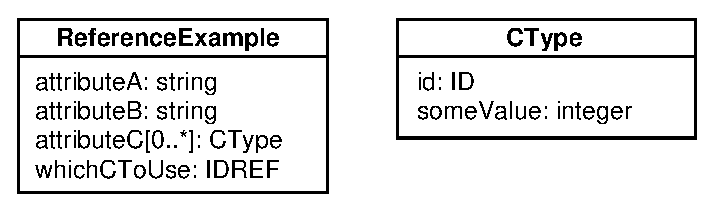
\includegraphics[scale = 0.7]{id-example.eps}
\end{center}
Here is an XML Schema to match the above:
\begin{small}
  \tightspacing
\begin{verbatim}
    <xsd:schema xmlns:xsd="http://www.w3.org/1999/XMLSchema">
    
    <xsd:complexType name="CType">
      <xsd:attribute name="id"        type="xsd:IDREF"/>
      <xsd:attribute name="someValue" type="xsd:integer"/>
    </xsd:complexType>

    <xsd:complexType name="SillyClass">
      <xsd:attribute name="attributeA" type="xsd:string"/>
      <xsd:attribute name="attributeB" type="xsd:string"/>
      <xsd:element   name="listOfC" minOccurs="1" maxOccurs="1">
        <xsd:complexType>
          <xsd:element name="CType" type="CType" minOccurs="0" maxOccurs="*"/>
        </xsd:complexType>
      </xsd:element>
      <xsd:attribute name="whichCToUse" type="xsd:IDREF"/>
    </xsd:complexType>

    </xsd:schema>
\end{verbatim}
  \regularspacing
\end{small}

It is worth noting in passing that this approach can be used to represent
graph structures in XML.  It is sometimes thought that XML can only be used
to represent tree-structured information.  But in fact, by assigning
\class{ID} type identifiers to different elements in a data structure, it
is possible to have elements link to each other and thereby allow full
graph-structured data to be represented.


%-----------------------------------------------------------------------------
\subsection{Link Attributes (For Inter-Object Links)}
%-----------------------------------------------------------------------------

Links need to be expressed not only between parts of the same object, but
between separate database objects as well.  This section treats this second
case.

UML notation does not make a clear distinction between a pointer to an
instance, and actual incorporation of the instance into an object.  To make
this clear in the presentation notation, we take the approach of defining a
new class for each link type.  The naming convention is to name the link
type according to the pattern \class{LinkTo}\rule{0.75in}{0.5pt}, where the
blank is replaced by the name of the object class.  For example, a link to
a \class{CellModel} object would be implemented using a type called
\class{LinkToCellModel}.

In XML, links can be implemented using the \emph{XML Linking Language},
XLink~(DeRose et al., 2000).  XLink is specifically designed for describing
links between separate resources.  For the limited applications that are
the domain of the present document, only the ``simple'' XLink type is
required.  This has the form shown in the following example:
\begin{small}
  \tightspacing
\begin{verbatim}
     ...
     <authors>
       <LinkToAuthor xlink:href="http://myserver.net/db/Author23"/>
       <LinkToAuthor xlink:href="http://myserver.net/db/Author24"/>
       <LinkToAuthor xlink:href="http://myserver.net/db/Author25"/>
       <LinkToAuthor xlink:href="http://myserver.net/db/Author26"/>
     </authors>
     ...
\end{verbatim}
  \regularspacing
\end{small}
The key ingredient in this example is the \attrib{xlink:href} attribute.
This is defined by XLink for use with simple links.  (There are additional
attributes that need to be specified when using XLink, but their values can
be set to common defaults in a XML Schema definition.)  The form of the
value of the \attrib{href} reference target (the four strings
``\texttt{http://....}''  in the example above) will depend on the
particular server storing the database, but the form will generally be a
URL as shown above.

When translating the UML-based notation into XML, the implementation of a
\class{LinkTo}\rule{0.75in}{0.5pt} type must use XLink syntax.  Although it
is not possible to define all possible link types here---the list of
possible types depends on the specific types defined in a particular
application---the following example XML Schema should give a sense for the
approach:
\begin{small}
  \tightspacing
\begin{verbatim}
    <xsd:schema xmlns:xsd="http://www.w3.org/1999/XMLSchema"
                xmlns:xlink="http://www.w3.org/2000/xlink">
    
    <xsd:complexType name="LinkToAuthor">
      <xsd:attribute name="xlink:type" type="string" value="simple" use="default"/>
      <xsd:attribute name="xlink:href" type="string"/>
    </xsd:complexType>

    <xsd:complexType name="SomeClass">

      <!-- ... other definitions presumably go here ...>

      <xsd:element   name="authors" minOccurs="1" maxOccurs="1">
        <xsd:complexType>
          <xsd:element name="LinkToAuthor" type="LinkToAuthor" minOccurs="0" maxOccurs="*"/>
        </xsd:complexType>
      </xsd:element>

      <!-- ... other definitions presumably go here ...>

    </xsd:complexType>

    </xsd:schema>
\end{verbatim}
  \regularspacing
\end{small}

There is one last detail worth mentioning.  The use of \attrib{xlink:href}
in an XML data stream requires the namespace for XLink to be declared.  In
the example above, this is done using the line that begins with
\texttt{xmlns:xlink=}.


%-----------------------------------------------------------------------------
\subsection{List Attribute}
\label{sub:list-attributes}
%-----------------------------------------------------------------------------

An attribute can be a list of simple types, or a list of complex types,
or a list of links.  All items in the list must have the same type.  In
some programming languages, a list might be represented as a vector.
\begin{wrapfigure}[11]{r}{2.25 in}
  \begin{center}
    \begin{tabular}{rl}
      1 & exactly one\\
      0,1 & zero or one\\
      0..4 & between zero and four\\
      3,7 & either three or seven\\
      0..* & zero or more\\
      \textrm{*} & zero or more\\
      1..* & one or more
    \end{tabular}
  \end{center}
\end{wrapfigure}
Lists are textually expressed using a notation loosely based on C and
Java-style array notation, with a multiplicity specifier enclosed in square
brackets.  The form of the specification of multiplicity consists of
numerals or the asterisk character, optionally separated by commas or `..'
(the last to indicate range).  Asterisk means ``zero or more''.  For
example, ``\attrib{somevar: Integer[10]}'' means that \attrib{somevar} is a
list of ten integers.  Similarly, ``\attrib{author: LinkToAuthor[1..*]}''
means that attribute \attrib{author} is a list of one or more links to
other \mbox{objects} in the database (in this case, \class{Author} objects,
although this is not explicit in the notation itself and relies on having
defined \class{LinkToAuthor} appropriately).  The table at the right gives
a number of other examples of multiplicity specifications.

Multiplicity involving complex types (as opposed to simple types) is
expressed in UML with numerals on the links joining two classes together.
For example, if in the \class{MyClass} example above, \attrib{attributeC}
had actually been a list of zero or more \class{AttrCType} structures
(i.e., if the declaration had been \attrib{attributeC: AttrCType[0..*]}),
then the corresponding UML diagram would be:

\begin{center}
  \figNB[scale = 0.7]{someschema-uml-multiple.eps}
\end{center}

By convention, if the relationship is 1-to-1, the two numeral 1's are
normally omitted from the association line in the UML diagram.  The absence
of any numerals on either end of an association line implies 1.

To get a sense for what an actual object might look like, suppose there
exists an instance of a \class{MyClass} object that has three elements in
\attrib{attributeC}.  Written in a C or Java-like programming language,
this might look like the following:
\begin{small}
\tightspacing
\begin{verbatim}
    obj.attributeA                        = "foo";
    obj.attributeB                        = "bar";

    obj.attributeC[0].anotherAttribute    = 1;
    obj.attributeC[0].yetAnotherAttribute = 2.2;

    obj.attributeC[1].anotherAttribute    = 5;
    obj.attributeC[1].yetAnotherAttribute = 12.0;

    obj.attributeC[2].anotherAttribute    = 30;
    obj.attributeC[2].yetAnotherAttribute = 40.23;
\end{verbatim}
\regularspacing
\end{small}
And now, the same object encoded in XML:
\begin{small}
  \tightspacing
\begin{verbatim}
    <MyClass attributeA="foo" attributeB="bar">
      <attributeC>
        <AttrCType anotherAttribute="1" yetAnotherAttribute="2.2"/>
        <AttrCType anotherAttribute="5" yetAnotherAttribute="12.0"/>
        <AttrCType anotherAttribute="30" yetAnotherAttribute="40.23"/>
      </attributeC>
    </MyClass>
\end{verbatim}
  \regularspacing
\end{small}

Finally, to illustrate how this would be translated into XML Schema, the
following shows a translation of the UML diagram above.  This is
essentially identical to the XML Schema given in
Section~\ref{sub:complex-attributes}, but with a change to the
\attrib{maxOccurs} property on the \class{AttrCType} subelement to allow an
unlimited number of them within \attrib{attributeC}.
  
\begin{small}
  \tightspacing
\begin{verbatim}
    <xsd:schema xmlns:xsd="http://www.w3.org/1999/XMLSchema">
    
    <xsd:complexType name="AttrCType">
      <xsd:attribute name="anotherAttribute"    type="xsd:integer"/>
      <xsd:attribute name="yetAnotherAttribute" type="xsd:float"/>
    </xsd:complexType>
    
    <xsd:attribute name="attributeA" type="xsd:string"/>
    <xsd:attribute name="attributeB" type="xsd:string"/>
    <xsd:element   name="attributeC" minOccurs="1" maxOccurs="1">
      <xsd:complexType>
        <xsd:element name="AttrCType" type="AttrCType" minOccurs="0" maxOccurs="*"/>
      </xsd:complexType>
    </xsd:element>
    
    </xsd:schema>
\end{verbatim}
  \regularspacing
\end{small}


%-----------------------------------------------------------------------------
\subsection{Constraints on Attribute Values}
%-----------------------------------------------------------------------------

It is often useful to be able to express constraints on the values of
attributes.  A constraint refers to a limitation or restriction on the
possible content or state of an attribute.  For example, it may be useful
to specify that a given integer attribute cannot have a value less than
zero, or that a given string attribute can only take on values from a
limited vocabulary.  UML has a standard notation for expressing
constraints; it consists of either adding a constraint expression in curly
braces following the definition of an attribute, as in the UML shown in the
following example:

\begin{center}
  \setlength{\tabcolsep}{40 pt}
  \tightspacing
  \small
  \begin{tabular}{@{}cc@{}}
    \begin{minipage}[b]{2 in}
      \begin{tabbing}
        attrBxx\=integerxx\=\kill
        \class{AnotherClass}\\
        \rule[0.5 ex]{2.25 in}{0.005in}\\
        \attrib{attrA}:\>\attribtype{Integer}\>\attrib{\{attrA != 0\}}\\
        \attrib{attrB}:\>\attribtype{String}\>\attrib{\{``val1'', ``val2'', ``val3''\}}\\
        \attrib{attrC}:\>\attribtype{String}
      \end{tabbing}
      \emph{Textual form}
    \end{minipage}
  &
    \begin{minipage}[b]{2 in}
      \figNB[scale = 0.7]{someschema-constraints.eps}\newline
      \emph{UML form}
    \end{minipage}
  \end{tabular}
  \regularspacing
\end{center}

Alternatively, in a UML diagram, the constraints can be placed in an
external text box and a line can be drawn from the box to the attribute in
question, as in the following:

\begin{center}
  \figNB[scale = 0.7]{someschema-constraints-boxed.eps}
\end{center}

%One situation arises frequently in data representations, and that is the
%need to constrain the values of a string attribute to be taken from a
%partially or fully constrained vocabulary.  We use the following notation
%to express different kinds of constraints in this context:
%\begin{itemize}
  
%\item If a string attribute's value should be a single string chosen only
%  from a strictly limited vocabulary (known as a controlled vocabulary),
%  the possible values are listed in curly braces next to the attribute:
%  \begin{quote}
%    \small
%    \tightspacing
%    \begin{tabbing}
%      Stringxxx\=attrbxxx\=\kill
%      \class{SomeSchema}\\
%      \rule[0.5 ex]{2.85 in}{0.005in}\\
%      \attrib{attrA}:\>\attribtype{String}\>\attrib{\{``val1'', ``val2'', ``val3''\}}
%    \end{tabbing}
%    \regularspacing
%  \end{quote}
  
%\item If a string attribute's value can be any single string, but the user
%  is to be provided with a list of suggested preferred values (i.e., the
%  vocabulary is partially controlled), the known preferred values are
%  listed in curly braces and an asterisk character is added at the end of
%  the list to indicate any other value is permitted as well:
%  \begin{quote}
%    \small
%    \tightspacing
%    \begin{tabbing}
%      Stringxxx\=attrbxxx\=\kill
%      \class{SomeSchema}\\
%      \rule[0.5 ex]{3.25 in}{0.005in}\\
%      \attrib{attrA}:\>\attribtype{String}\>\attrib{\{``val1'', ``val2'', ``val3'', *\}}
%    \end{tabbing}
%    \regularspacing
%  \end{quote}
  
%\item If a string attribute's value can be one or more strings chosen from
%  either a controlled vocabulary or a partially controlled vocabulary, the
%  constraint is expressed as follows:
%  \begin{quote}
%    \small
%    \tightspacing
%    \begin{tabbing}
%      Stringxxx\=attrbxxx\=\kill
%      \class{SomeSchema}\\
%      \rule[0.5 ex]{4.5 in}{0.005in}\\
%      \attrib{attrA}:\>\attribtype{String}\>\attrib{\{one or more of: ``val1'', ``val2'', ``val3''\}}\\
%      \attrib{attrB}:\>\attribtype{String}\>\attrib{\{one or more of: ``valA'', ``valB'', ``valC'', *\}}
%    \end{tabbing}
%    \regularspacing
%  \end{quote}
%  This particular form (the use of the string ``one or more of'') is not
%  defined in UML; it is a simple extension introduced as part of the
%  notation being described here.

%\end{itemize}

XML Schema defines several mechanisms for constraining values of
attributes.  A particularly useful one is the \attrib{enumeration}
component.  Here is an example of an XML Schema constraining the values of
an attribute to a set of specific strings:
\begin{small}
  \tightspacing
\begin{verbatim}
    <xsd:schema xmlns:xsd="http://www.w3.org/1999/XMLSchema">
    
    <xsd:complexType name="TotallyDifferentExample">
      <xsd:attribute name="theVariable">
        <xsd:simpleType base="xsd:string">
          <xsd:enumeration value="value1"/>
          <xsd:enumeration value="value2"/>
          <xsd:enumeration value="value3"/>
        </xsd:simpleType>
      </xsd:element>
    </xsd:complexType>
    
    </xsd:schema>
\end{verbatim}
  \regularspacing
\end{small}


%-----------------------------------------------------------------------------
\subsection{Inheritance}
%-----------------------------------------------------------------------------

Inheritance allows a class to be defined as an extension or derivation of
another class.  In textual form, the inheritance relationship can be
written on the same line as the name of the class definition; in graphical
UML form, inheritance is expressed using an open-ended arrow drawn from an
inheriting class to the inherited-from class.  The following illustrates
both forms:

\begin{center}
  \tightspacing
  \small
  \setlength{\tabcolsep}{30 pt}
  \begin{tabular}{@{}cc@{}}
    \begin{minipage}[b]{1.6in}
      \begin{tabbing}
        Stringxxx\=attrbxxx\=\kill
        \class{SomeClass extends SomeOtherClass}\\
        \rule[0.5 ex]{2.25 in}{0.005in}\\
        \attrib{attrA}:\>\attribtype{String}
      \end{tabbing}
      \emph{Text form}
    \end{minipage}
    & 
    \begin{minipage}[b]{2 in}
      \figNB[scale = 0.7]{someschema-inherit.eps}\newline
      \emph{UML form}
    \end{minipage}
  \end{tabular}
  \regularspacing
\end{center}

The meaning of the above is that \class{SomeClass} has as attributes
\emph{both} \attrib{attrA} and \attrib{myValue}.  \class{SomeOtherClass}
has only one attribute, \attrib{myValue}.

In XML, inheritance can be implemented using the \attrib{derivedBy}
mechanism.  This allows an XML element/class definition to be based on
another element.  Here is an XML Schema definition for the example above:
\begin{small}
  \tightspacing
\begin{verbatim}
    <xsd:schema xmlns:xsd="http://www.w3.org/1999/XMLSchema">
    
    <xsd:complexType name="SomeOtherClass">
      <xsd:attribute name="myValue" type="xsd:string"/>
    </xsd:complexType>

    <xsd:complexType name="SomeClass" base="SomeOtherClass" derivedBy="extension">
      <xsd:attribute name="attrA" type="xsd:string"/>
    </xsd:complexType>

    </xsd:schema>
\end{verbatim}
  \regularspacing
\end{small}

%=============================================================================
\subsection{Specifying Units}
%=============================================================================

It is often important to provide information about the units associated
with a numerical attribute.  In the approach to XML representations used
here, there are two alternatives for specifying units conveniently.

The first approach is to define, for each relevant attribute, another
attribute whose name has the suffix \attrib{\_units} and whose type is a
string, to represent the units being used for the value stored in the
attribute.  The following is an example:
\begin{center}
  \tightspacing
  \small
  \setlength{\tabcolsep}{30 pt}
  \begin{tabular}{@{}ll@{}}
    \begin{minipage}[b]{1.3 in}
      \raisebox{-2ex}{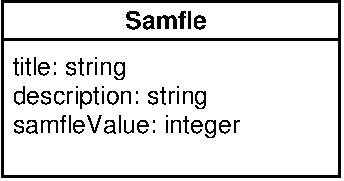
\includegraphics[scale = 0.7]{sampleschema-units.eps}}
    \end{minipage}
  &
    \begin{minipage}[b]{3 in}
      \begin{tabbing}
        xx\=\kill
        \verb|<complexType name="Sample">|\\
        \>\verb|<attribute name="title" type="string"/>|\\
        \>\verb|<attribute name="description" type="string"/>|\\
        \>\verb|<attribute name="sampleValue" type="integer"/>|\\
        \>\verb|<attribute name="sampleValue_units" type="string"/>|\\
        \verb|</complexType>|
      \end{tabbing}
    \end{minipage}
    \\
    \\
    \emph{UML Form} & \emph{XML Schema}
  \end{tabular}
  \regularspacing
\end{center}

The second approach is suitable for groups of attributes or substructures
that all use the same unit.  In that case, it may be simpler to use an
attribute at the class level that sets the units for a whole object.

In order to maximize the utility of having unit specifications, a given
project (such as the ERATO Kitano Systems Biology Project) should define a
specific XML type for the units it needs to use.  This specification should
take the form of a data type (perhaps called \class{Units}), defined in a
separate XML Schema, consisting of an enumeration of strings that can
appear as unit specifications in other Schemas.  Here is a partial example
of such an XML Schema:
\begin{small}
  \tightspacing
\begin{verbatim}
    <xsd:schema xmlns:xsd="http://www.w3.org/1999/XMLSchema">
    
    <xsd:simpleType name="Units" base="xsd:string">
      <xsd:enumeration value="m"/>
      <xsd:enumeration value="cm"/>
      <xsd:enumeration value="mm"/>

      <!-- and so on ... -->

    </xsd:simpleType>

    </xsd:schema>
\end{verbatim}
  \regularspacing
\end{small}



%=============================================================================
\section{Summary}
%=============================================================================

The notation proposed in this document is a subset of what could be used
and what UML provides.  The subset was chosen to be as simple as possible
yet allow the expression of the kinds of data structures that need to be
encoded in XML for systems biology.  The notation proposed here is not
carved in stone, and will undoubtedly continue to evolve.  Please use the
project email address (\texttt{sysbio@caltech.edu}) to send your
comments and suggestions on this proposal.


%=============================================================================
\section{References}
%=============================================================================

% FIXME: add web refs for the hucka et al papers.

\setlength{\parskip}{1.2ex}

\begin{flushleft}

Biron, P.~V., and Malhotra, A.  (2000).  XML Schema Part 2: Datatypes (W3C
Working Draft 7 April 2000).  Available via the World Wide Web at
\url{http://www.w3.org/TR/xmlschema-2/}.

Bosak, J., and Bray, T. (1999).  {XML} and the Second-Generation Web.
Scientific American, May.  Also available via the World Wide Web at
\url{http://www.sciam.com/1999/0599issue/0599bosak.html}.

Bray, T. (2000).  RE: When is an attribute an attribute?  Posting to the
\url{xml-dev} mailing list, Apr 1998.  Available via the World Wide Web at
\url{http://www.oasis-open.org/cover/brayAttr980409.html}.

Bray, T., Paoli, J., and Sperberg-McQueen, C.~M. (1998). Extensible Markup
Language (XML) 1.0, W3C Recommendation 10-February-1998.  Available via the
World Wide Web at \url{http://www.w3.org/TR/1998/REC-xml-19980210}.

Cover, R.  (2000).  SGML/XML Elements versus Attributes: When Should I Use
Elements, and When Should I Use Attributes?   Available via the World Wide
Web at \url{http://www.oasis-open.org/cover/elementsAndAttrs.html}.

DeRose, S., Maler, E., Orchard, D., and Trafford, B. (2000).  XML Linking
Language (XLink) Version 1.0 W3C Candidate Recommendation 3 July 2000.
Available via the World Wide Web at \url{http://www.w3.org/TR/xlink/}.

Eriksson, H.-E., and Penker, M. (1998).  UML Toolkit.  New York: John Wiley
\& Sons.

Fallside, D.~C.  (2000).  XML Schema Part 0: Primer (W3C Working Draft, 7
April 2000).  Available via the World Wide Web at
\url{http://www.w3.org/TR/xmlschema-0/}.

Oestereich, B.  (1999).  Developing Software with UML: Object-Oriented
Analysis and Design in Practice.  Addison-Wesley.

St. Laurent, S. (2000).  XML Elements of Style. 

Thompson, H.~S., Beech, D., Maloney, M., and Mendelsohn, N. (2000).  XML
Schema Part 1: Structures (W3C Working Draft 7 April 2000).  Available via
the World Wide Web at \url{http://www.w3.org/TR/xmlschema-1/}.

\end{flushleft}

\end{document}



%XML, the Extensible Markup Language (Bosak and Bray, 1999; Bray, Paoli and
%Sperberg-McQueen, 1998) is a language used to express self-describing,
%structured representations of information.  It provides a way of marking up
%data with semantic tags that describe and structure the contents of the
%data.  Although XML is typically thought of as a document format similar to
%HTML, in fact it is more general.  It is a notation, a ``metalanguage'', a
%way of organizing a stream of data and marking up the different parts so
%that a program can parse the stream into constituents.  In the words of one
%of its chief architects, ``Just as HTML created a way for every computer
%user to read Internet documents, XML makes it possible, despite the Babel
%of incompatible computer systems, to create an Esperanto that all can read
%and write.  Unlike most computer data formats, XML markup also makes sense
%to humans, because it consists of nothing more than ordinary text''~(Bosak
%and Bray, 1999).
